\documentclass{article}

\usepackage{amsmath, amsthm, amssymb, amsfonts}
\usepackage{thmtools}
\usepackage{graphicx}
\usepackage{setspace}
\usepackage{geometry}
\usepackage{float}
\usepackage{hyperref}
\usepackage[utf8]{inputenc}
\usepackage[english]{babel}
\usepackage{framed}
\usepackage[dvipsnames]{xcolor}
\usepackage{tcolorbox}
\usepackage{mathrsfs}
\usepackage{bbm}
\usepackage{dsfont} % For the indicator function \mathds{1}

\colorlet{LightGray}{White!90!Periwinkle}
\colorlet{LightOrange}{Orange!15}
\colorlet{LightGreen}{Green!15}
\colorlet{LightBlue}{Blue!15}

\newcommand{\HRule}[1]{\rule{\linewidth}{#1}}

\declaretheoremstyle[name=Theorem,]{thmsty}
\declaretheorem[style=thmsty,numberwithin=section]{theorem}
\tcolorboxenvironment{theorem}{colback=LightGray}

\declaretheoremstyle[name=Proposition,]{prosty}
\declaretheorem[style=prosty,numberlike=theorem]{proposition}
\tcolorboxenvironment{proposition}{colback=LightOrange}

\declaretheoremstyle[name=Definition,]{prcpsty}
\declaretheorem[style=prcpsty,numberlike=theorem]{definition}
\tcolorboxenvironment{definition}{colback=LightGreen}

\declaretheoremstyle[name=Remark,]{prosty}
\declaretheorem[style=prosty,numberlike=theorem]{remark}
\tcolorboxenvironment{remark}{colback=LightBlue}

\setstretch{1.2}
\geometry{
    textheight=9in,
    textwidth=5.5in,
    top=1in,
    headheight=12pt,
    headsep=25pt,
    footskip=30pt
}

% ------------------------------------------------------------------------------

\begin{document}

% ------------------------------------------------------------------------------
% Cover Page and ToC
% ------------------------------------------------------------------------------

\title{ \normalsize \textsc{}
		\\ [2.0cm]
		\HRule{1.5pt} \\
		\LARGE \textbf{\uppercase{FIN 417: Quantitative Risk Management}
		\HRule{2.0pt} \\ [0.6cm] \LARGE{Rafiki's Notes} \vspace*{10\baselineskip}}
		}
\date{}
\author{\textbf{Rafael Barroso} \\ 
		Ingenierie Mathematique \\
		École Polytechnique Fédérale de Lausanne \\
		\today}

\maketitle
\newpage

\tableofcontents
\newpage

% ------------------------------------------------------------------------------

\section{Basic notions} \label{sec:part1}
We first start by exploring some basic notions of risk, and mainly define all of the financial jargon that is used throughout the course.

\subsection{Financial risk and regulation}
There are a lot of definitions of risk, but as for many things in life, no sentence can capture the full essence of a concept (especially in finance since all of the theory is constructed by phony, try-harding beaurocrats i.e. beaurocs).
As such, we will just list some of the most common definitions of risk:

\vspace{0.2cm}

\begin{itemize}
    \item The Concise Oxford English Dictionary: `hazard, a chance of bad consequences, loss or exposure to mischance'.
    \item The course textbook (M.F.E. McNeil, R. Frey, P. Embrechts, Quantitative Risk Management: Concepts, Techniques and Tools, Princeton University Press, 2015): `any event or action that may adversely affect an organization's ability to achieve 
    its objectives and execute its strategies'.
    \item ISO 31073: ` efect of uncertainty on objectives; can be positive, negative or both, can result in opportunities and threats'. This same guide also defines: 
    \begin{itemize}
        \item \textbf{Uncertainty}: state, even partial, of deficiency of information related to understanding or knowledge (`randomness').
        \item \textbf{Objective}: result to be achieved.
        \item \textbf{Risk management}: coordinated activities to direct and control an organization with regard to risk.
    \end{itemize}
\end{itemize}

\vspace{0.2cm}

As you can see, pure jargon and buzzwords are used to define risk, which is not very helpful. In this course we define risk as the following notion.

\begin{definition}
    Risk is the chance of financial loss due to uncertainty or `randomness' (but what is randomness anyway? don't even ask cuz' I get erected).
\end{definition}

So, given this defintion, we may model and measure risk using probabilistic (i.g. random variables, distributions) and statistical (i.g. data) tools, which is what we will do in this course. Mainly, we may thank daddy Kolmogorov for developing
a reliable mathematical framework (using probabilistic axioms) to think about risk in a rigorous manner. Since this course is heavily focused on finance, we will mainly be concerned with financial risk, which, yoy guessed it, has a shit ton of
variable definitions (each focusing on diferent aspects of finance).

\begin{remark}
    Note that financial risk is generated by a future change in value of an asset.
\end{remark}

\vspace{0.2cm}

Here are some of the main types of financial risk:

\begin{itemize}
    \item \textbf{Market risk}: change in value due to changes in underlying components (such as
    stock, bond, or commodity prices).
    \item \textbf{Credit risk}: possibility of not obtaining future payments due to fuck ups of the counterparty.
    \item \textbf{Operational risk}: risk of loss due to inadequate or failed internal process, people (beaurocs in action!) and systems  or from external events (fraud, earthquakes).
    \item \textbf{Liquidity risk}: not being able to buy or sell something quickly enoguh to minimize loss.
    \item \textbf{Model risk}: using an inadequate model for measuring risk.
\end{itemize}

\vspace{0.2cm}

Note that financial firms are not passive (i.e. defensive) towards risk, they confront it in order to gain return (risk tha biscuit!). Thus, Banks and insurers are like risk function engineers. They take raw random variables (risky outcomes), apply transformations $f(X)$,
 and then allocate these transformed versions to those most willing to hold them. That process is what keeps financial markets running smoothly.

 \begin{definition}
    A \textit{financial derivative} is a contract whose payoff is a function $f$ of some underlying random variable $U$ (e.g., stock price at time $T$). The whole industry is about analyzing, pricing, and hedging such contracts under uncertainty.
 \end{definition}

\newpage

\section{Standard risk measures and methods} \label{sec:part2}
After all of the jargon, we get into the good stuff. This section focuses on developing the framework we'll use later on in order to do some risk management.

\subsection*{Value and Loss}
We denote the value of a portfolio as $V$ (mathematically, a stochastic process) where at each time $t$ the value of the portfolio is defined as $V_t = V(t)$. Then,
each random variable $V(t)$ is observable at time $t$.

\begin{definition}
    For a given risk horizon $\Delta$, we define the loss of a portfolio $V$ over the period $ \left[ t, t + \Delta \right] $ as
    $$\mathcal{L}(t, t + \Delta) = - (V_{t + \Delta} - V_t)$$
    this is observable at time $t + \Delta$ but is `random' at $t$. This distribution is called the \textit{loss distribution}.
\end{definition}

\vspace{0.2cm}

A large positive value of $L$ indicates that the portfolio suffered a large decrease in value over $\left[ t, t + \Delta \right]$. We also define the \textbf{negative} of the loss function,
called the Profit-and-loss distribution i.e. $PnL(t, t + \Delta) = - \mathcal{L}(t, t + \Delta)$.

\begin{figure}[htbp]
\centerline{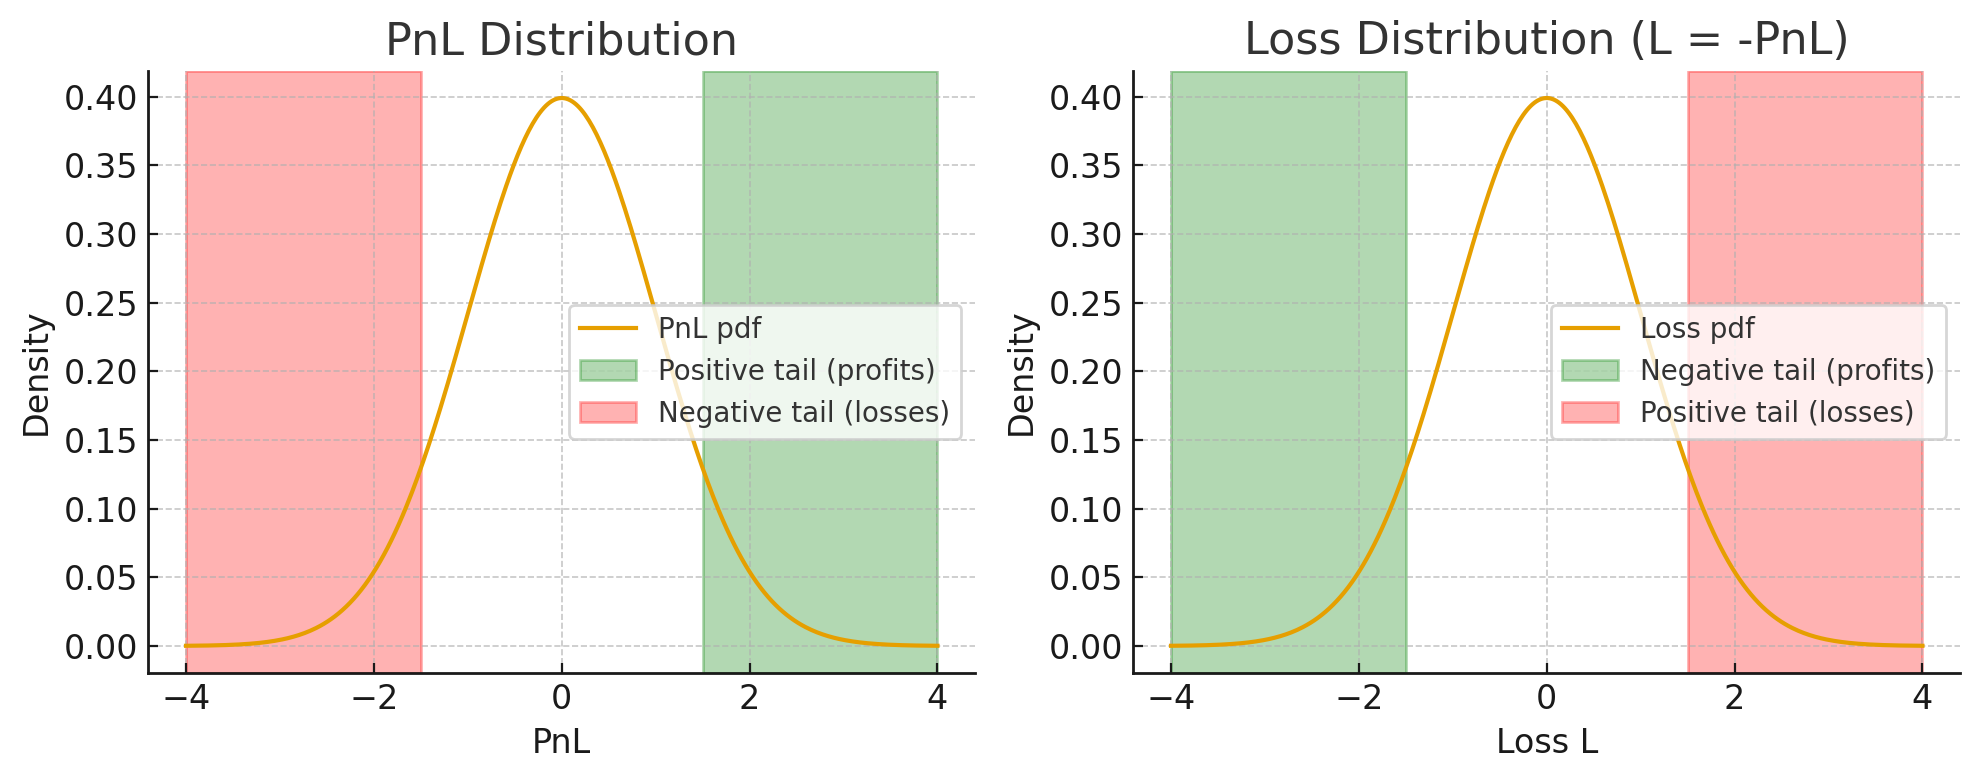
\includegraphics[scale=0.5]{figures/pnl_v_l_distributions.png}}
\caption{PnL v. Loss distribution}
\label{lossvpnl}
\end{figure}

\begin{remark}
    Much of risk management is focused on the negative tail of the PnL distribution, which is equivalent to the possitive tail of the loss distriution. 
\end{remark}

Sometimes, we may not have a full understanding (or any at all) of $\mathcal{L}$. It is also important to know that we may sometimes model $V$ as a function of
several risk factors. This suggests the following notation:

\begin{itemize}
    \item $V_t = f(t, Z_t)$: value of portfolio as function of underlying risk factors.
    \item $Z_t = (Z_{1,t}, \ldots, Z_{d, t})$: underlying risk factors; often representing stock value, intrest rate, etc.
    \item $f: \mathbb{R} \times \mathbb{R}^d \rightarrow \mathbb{R}$: measurable function.
    \item for $V_t$ to be observable at time $t$, we must have $Z_{k,t}$ observable at $t \text{  } \forall k$
\end{itemize}

The choice for each $Z_k$ and $f$ is a modeling issue.

\begin{definition}
    We define the vector of risk factor changes as $X_{t + \Delta} = Z_{t + \Delta} - Z_t$ and so, we may redefine the loss distribution as
    $$\mathcal{L}(t, t + \Delta) = - \left( V_{t + \Delta} - V_t \right) = - \left( f(t + \Delta, Z_{t + \Delta}) - f(t, Z_t) \right) $$
    $$\Rightarrow \mathcal{L} = - \left( f(t + \Delta, X_{t + \Delta} + Z_t) - f(t, Z_t) \right)$$
\end{definition}

The loss distribution is fully determined by the distribution of $X_{t + \Delta}$ and the function $f$. If $f$ is differentiable, we sometimes consider a first-order taylor approximation of the loss as
$$\mathcal{L}^{\delta}(t, t + \Delta) = - \left( \partial_t f(t, Z_t) \Delta + \sum_{i=1}^{d} \partial_{Z_i} f(t, Z_i)X_{i, t + \Delta} \right)$$

\begin{remark}
    Note that this aproximation is good whenever $\Delta$ is small enough. This may be observed in figure \ref{firstorderaprox}.
\end{remark}

\begin{figure}[htbp]
\centerline{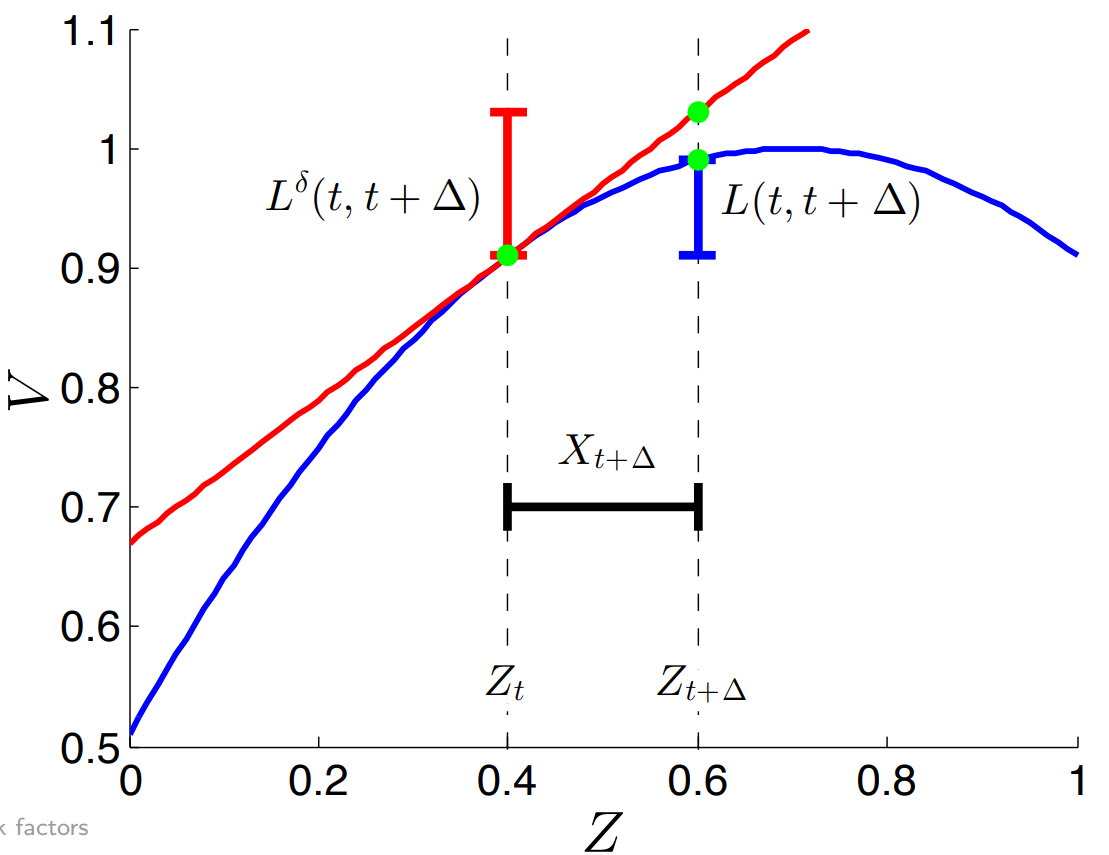
\includegraphics[scale=0.2]{figures/linear_approx_lossdistribution.png}}
\caption{First order Taylor aproximation of $\mathcal{L}$}
\label{firstorderaprox}
\end{figure}

\newpage

% ------------------------------------------------------------------------------
% Reference and Cited Works
% ------------------------------------------------------------------------------

\bibliographystyle{IEEEtran}
\bibliography{biblio.bib}

% ------------------------------------------------------------------------------

\end{document}
